\documentclass[12pt]{article}

\usepackage{geometry, subfiles}
\usepackage{amsmath, amssymb}
\usepackage{booktabs, longtable, siunitx}
\usepackage{graphicx}
\graphicspath{{/Users/wonjun/Dropbox/Emory/ECON771_health2/assignments/assignment1/output/}}

\title{Assignment 1}
\author{Wonjun Choi}

\begin{document}
\maketitle
	\begin{itemize}
		\item[1.] Provide and discuss a table of simple summary statistics showing the mean, standard deviation, min, and max of hospital total revenues and uncompensated care over time.
		
		The summary statistics of hospital total revenues and uncompensated care over time are presented in Table 1 and 2, respectively. All of the statistics are scaled by million dollar.
		\subfile{../output/tab_sumstat_rev}
		\subfile{../output/tab_sumstat_uncompcare}
		
		
		
		\item[2.] Create a figure showing the mean hospital uncompensated care from 2003 to 2019. Show this trend separately by hospital ownership type (private not for profit and private for profit).
		
		The mean hospital uncompensated care from 2003 to 2019 are shown in Figure 1.
		\begin{figure} [ht]
			\centering
			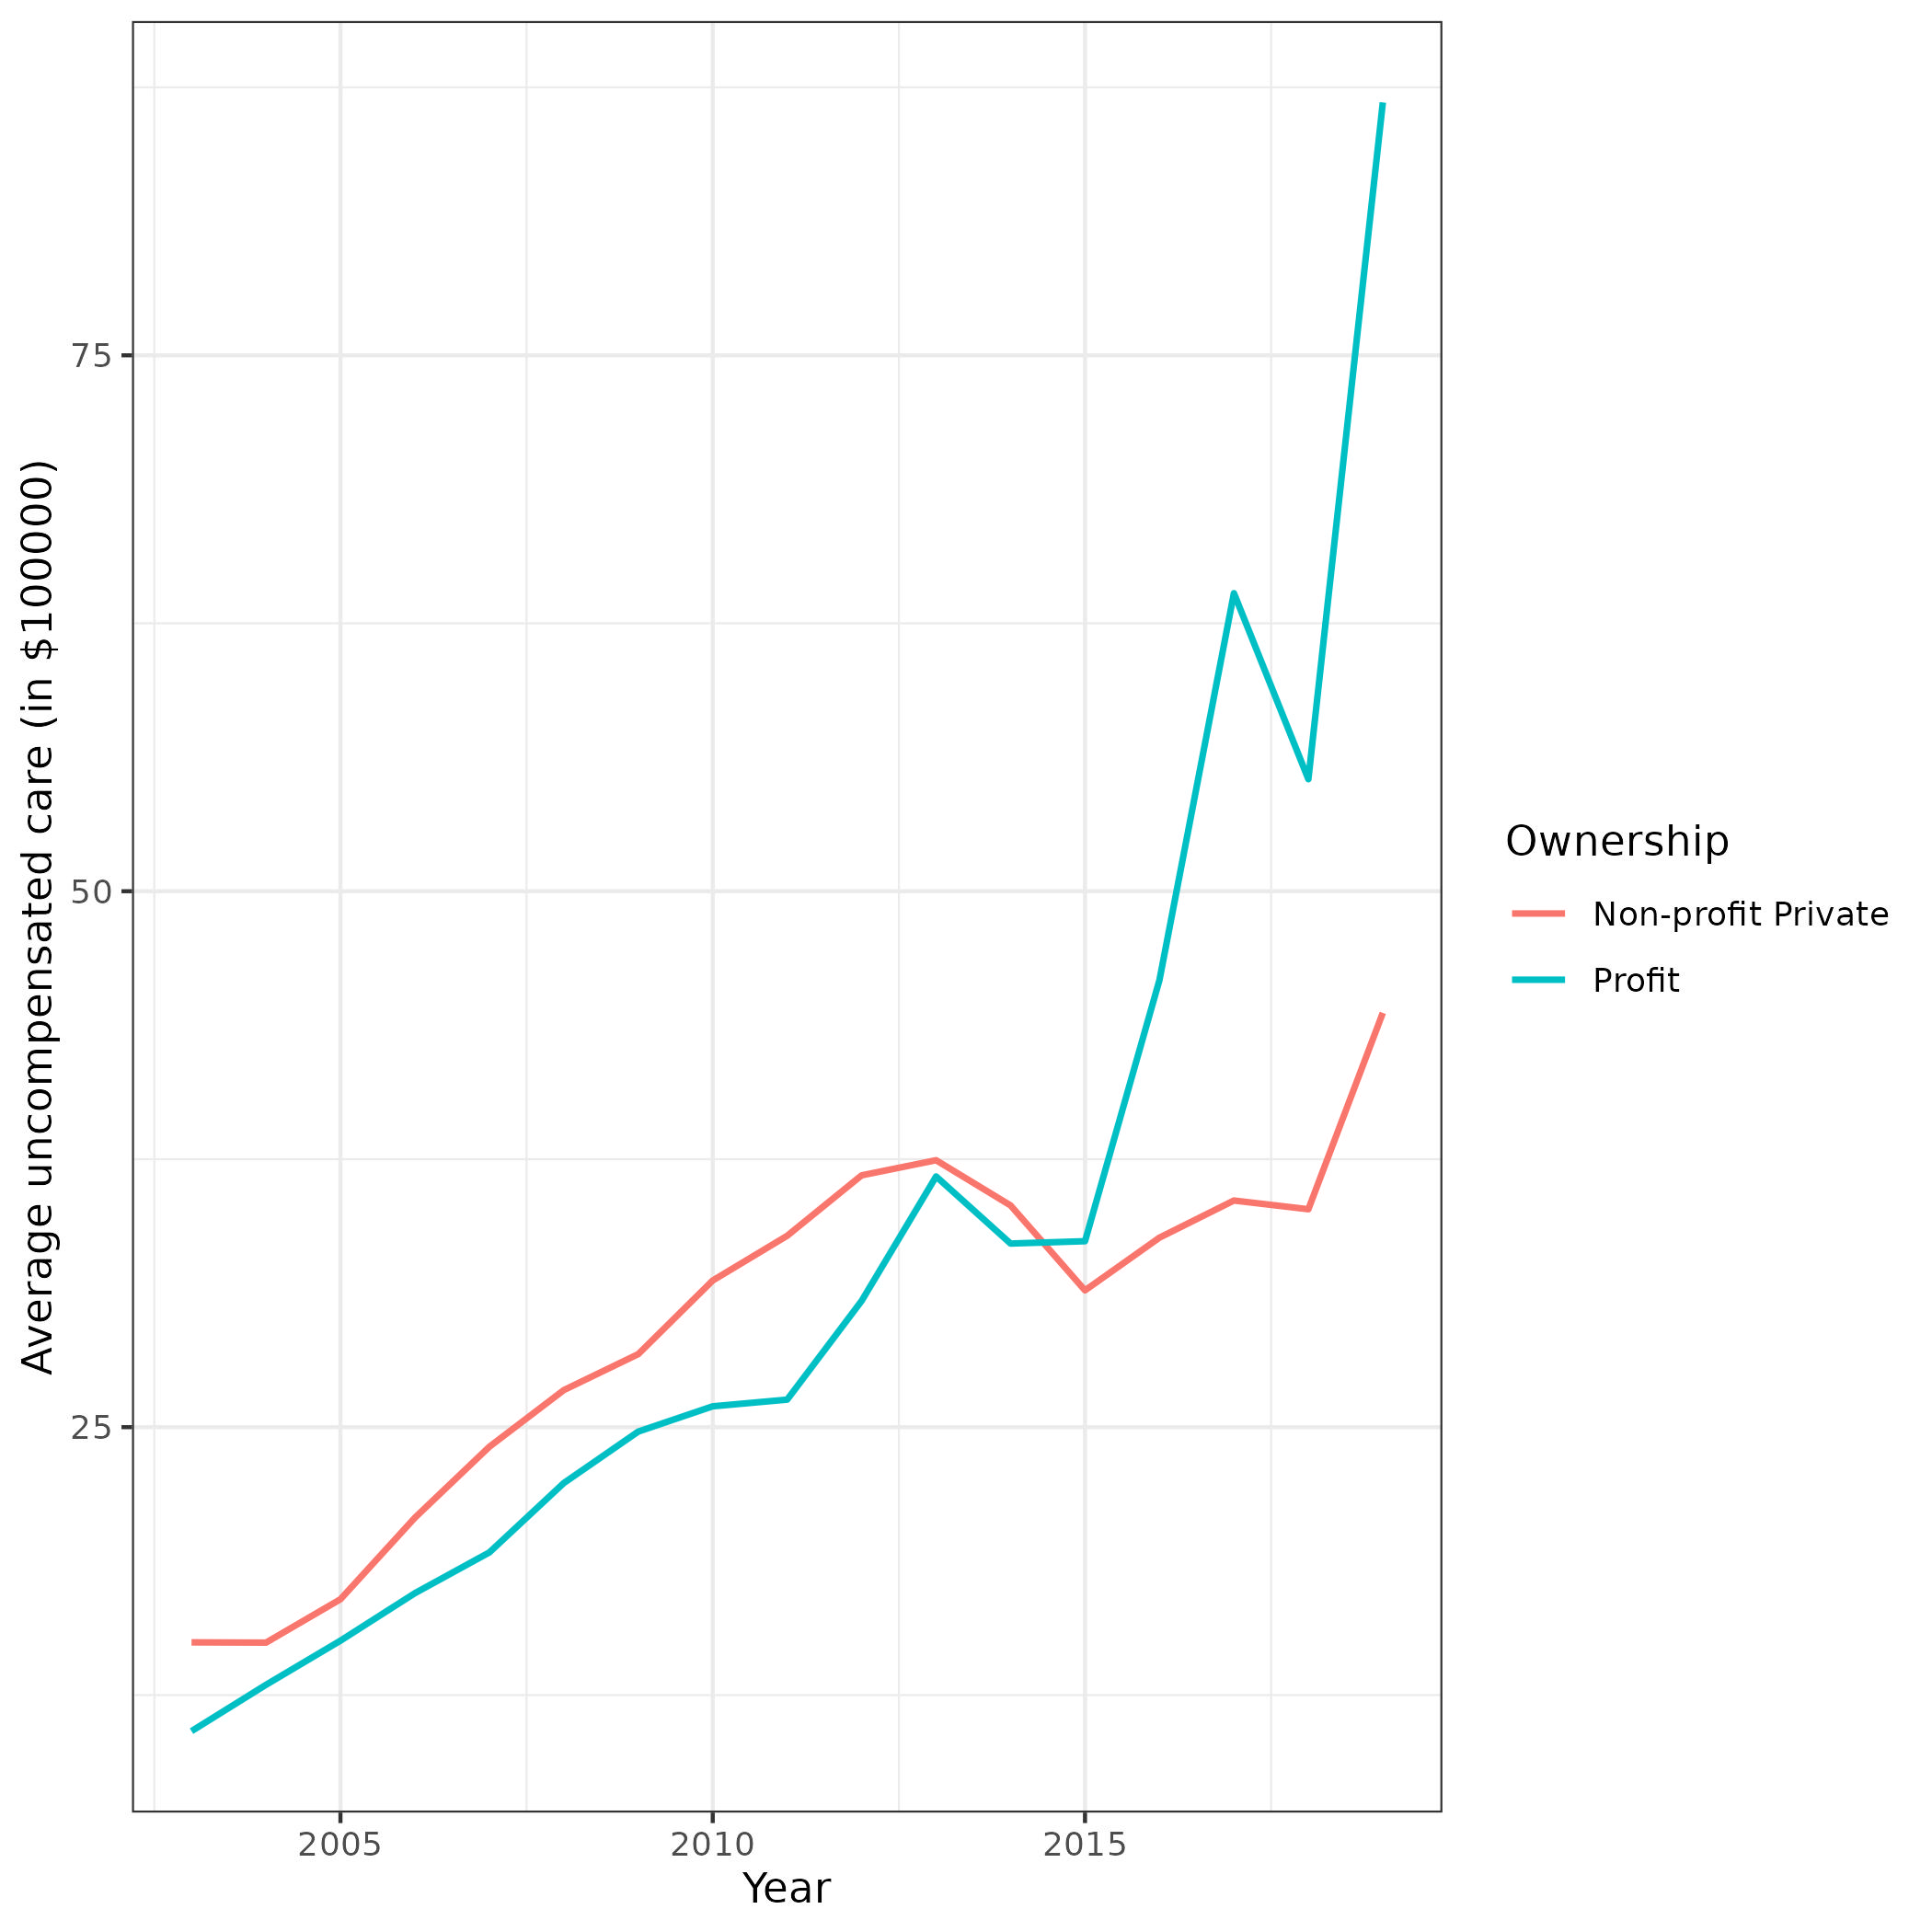
\includegraphics[scale=0.2]{fig_uncompcare.jpg}
			\caption{dd}
		\end{figure}
		Not-for-profit: haha
		For-profit: haha
		
		\item[3.] To estimate the effect of  Medicaid expansion on hospital uncompensated care, I estimate the following two-way fixed effects (TWFE) model.
		\begin{eqnarray}
			y_{it} = \alpha_i + \gamma_t + \delta D_{it} + \epsilon_{it}
		\end{eqnarray}
	    where $D_{it} = 1(E_i \le t)$, $E_i$ is an expansion year, $1(\cdot)$ is an indicator function. $\gamma_t$ denotes time fixed effects, $\alpha_i$ denotes hospital fixed effects, and $y_{it}$ denotes the hospital $i$’s amount of uncompensated care in year $t$.
	    
	    \subfile{../output/tab_twfe}
	    
	    The estimation results are presented in Table 3.  The first column is the result of the estimation using full sample. The coefficient suggests that the exansion of Medicade decreased hospital uncompensated care by 31 million dollars.
	    		
		\item[4.]
		
		\item[5.]
		
		\item[6.]
		\begin{figure}
			\centering
			  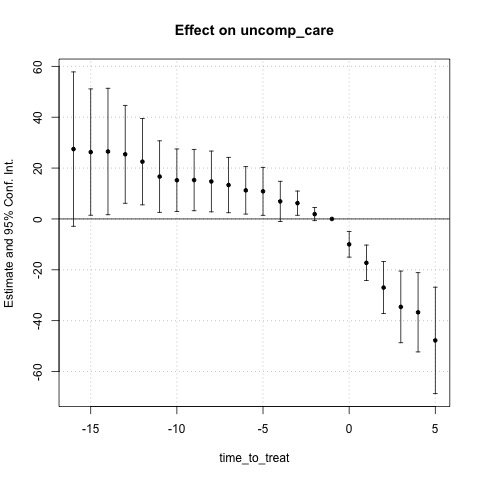
\includegraphics[scale=0.7]{fig_sunab.jpg}
			  \caption{dd}
		\end{figure}
		
		\item[7.]
		
		\item[8.]
		
		\item[9.]
		
		\item[10.]
	\end{itemize}
\end{document}